\section[ML overview]{Machine learning overview}

\subsection{}

\begin{frame}
    \frametitle{What is machine learning?}

    \begin{block}{My definition}
        The study of computational algorithms
        \begin{itemize}
            \item that \alert{predict} outputs or patterns from inputs;
            \item whose behavior is determined by \alert{model parameters};
            \item that \alert{learn} how to make predictions (``inference'')by fitting (``training'') the model parameters to data;
            \item that \alert{iteratively} improve their model parameters via continual training.
        \end{itemize}
    \end{block}
    \pause

    \begin{columns}
        \begin{column}{2.5in}
            Simplest example: linear regression
            \begin{itemize}
                \item Sort of: not iterative
                \item Predicts $y$ from $x$ via $y = ax + b$
                \item Two parameters: $a$, $b$
                \item Fitted to data
            \end{itemize}
        \end{column}
        \begin{column}{1.75in}
            \visible<+->{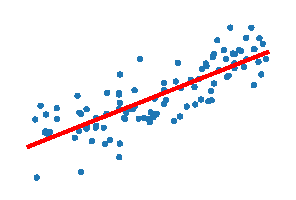
\includegraphics{linear_regression}}
        \end{column}
    \end{columns}
\end{frame}

\begin{frame}
    \frametitle{A (much) more complicated example}
    \begin{columns}
        \begin{column}{0.37\textwidth}
            \begin{block}{Image classification}
                A canonical problem: given an image, predict the correct label
            \end{block}
        \end{column}
        \begin{column}{0.63\textwidth}
            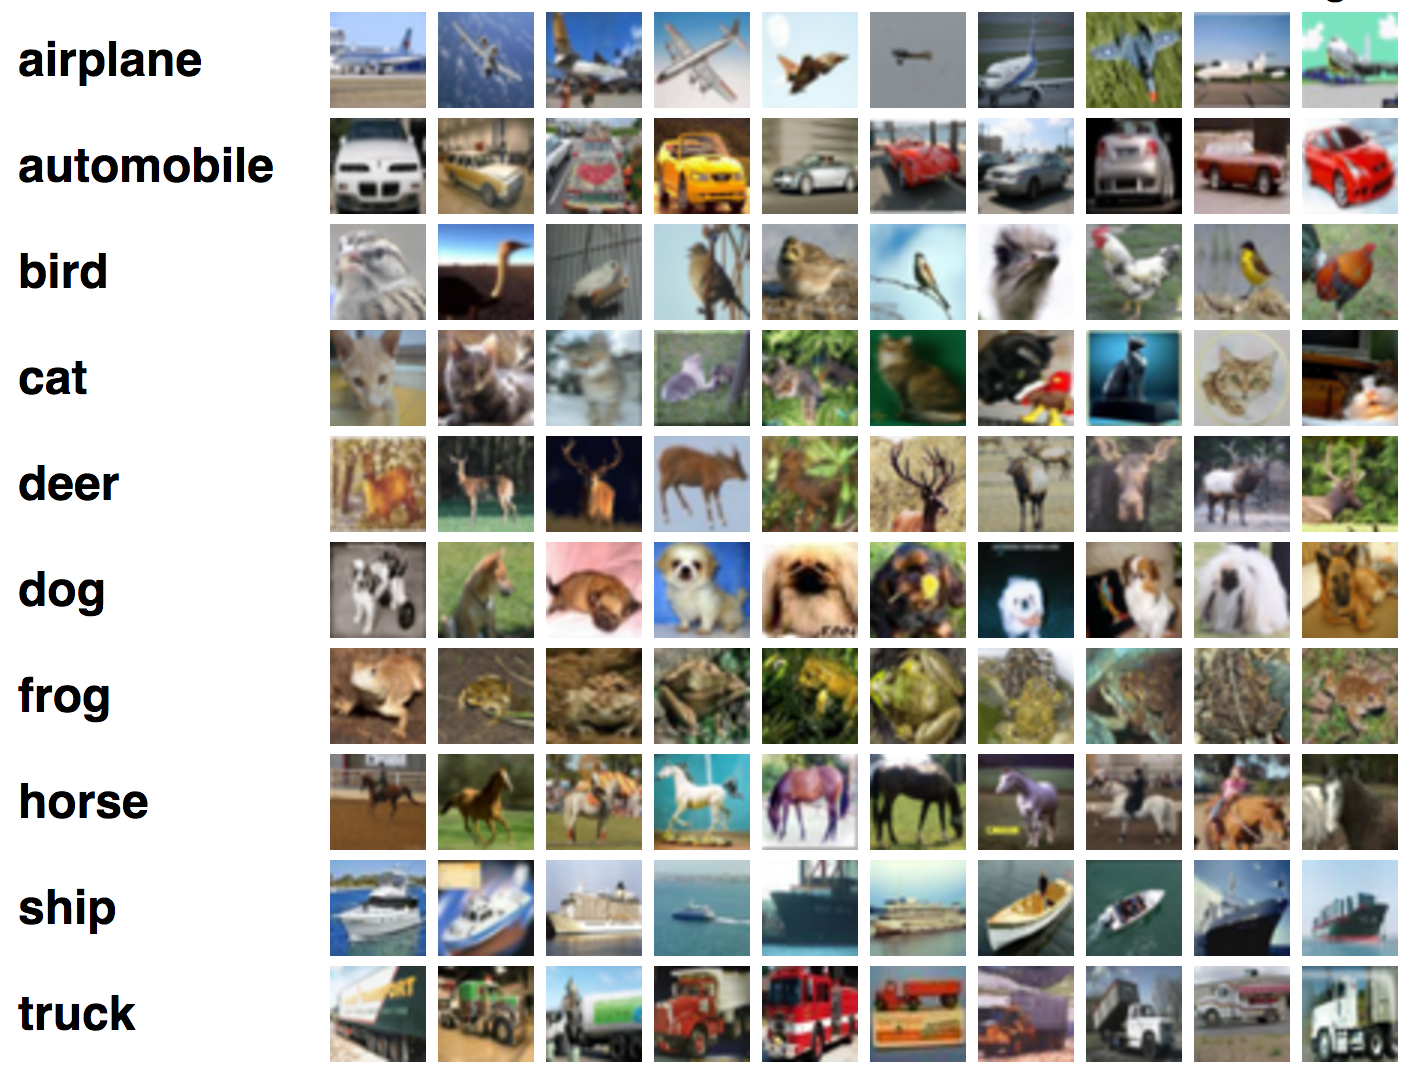
\includegraphics[width=\textwidth]{cifar10} \\
            \centering \footnotesize The CIFAR-10 problem
        \end{column}
    \end{columns}

    \begin{itemize}
        \item Roughly: if a human can do it, a computer should be able to too
        \item More rigorously: $\exists$ a mapping from image pixels to labels
        \begin{itemize}
            \item Mapping too difficult for humans to understand
            \item Let an algorithm model it
        \end{itemize}
    \end{itemize}
\end{frame}

\begin{frame}
    \frametitle{An image classification solution}

    \begin{columns}
        \begin{column}{0.7\textwidth}
            ResNet-152: a 152-layer convolutional neural network with 11.3 billion multiply/adds! \citep{He15b}
            \begin{itemize}
                \item Trained on ImageNet data: 14,197,122 images
                \item Iterative training
                \begin{itemize}
                    \item 600,000 training iterations
                    \item At each iteration, model parameters updated based on \emph{mini-batch} of 256 images
                \end{itemize}
                \item Won multiple image classification competitions
            \end{itemize}
        \end{column}
        \begin{column}{0.3\textwidth}
            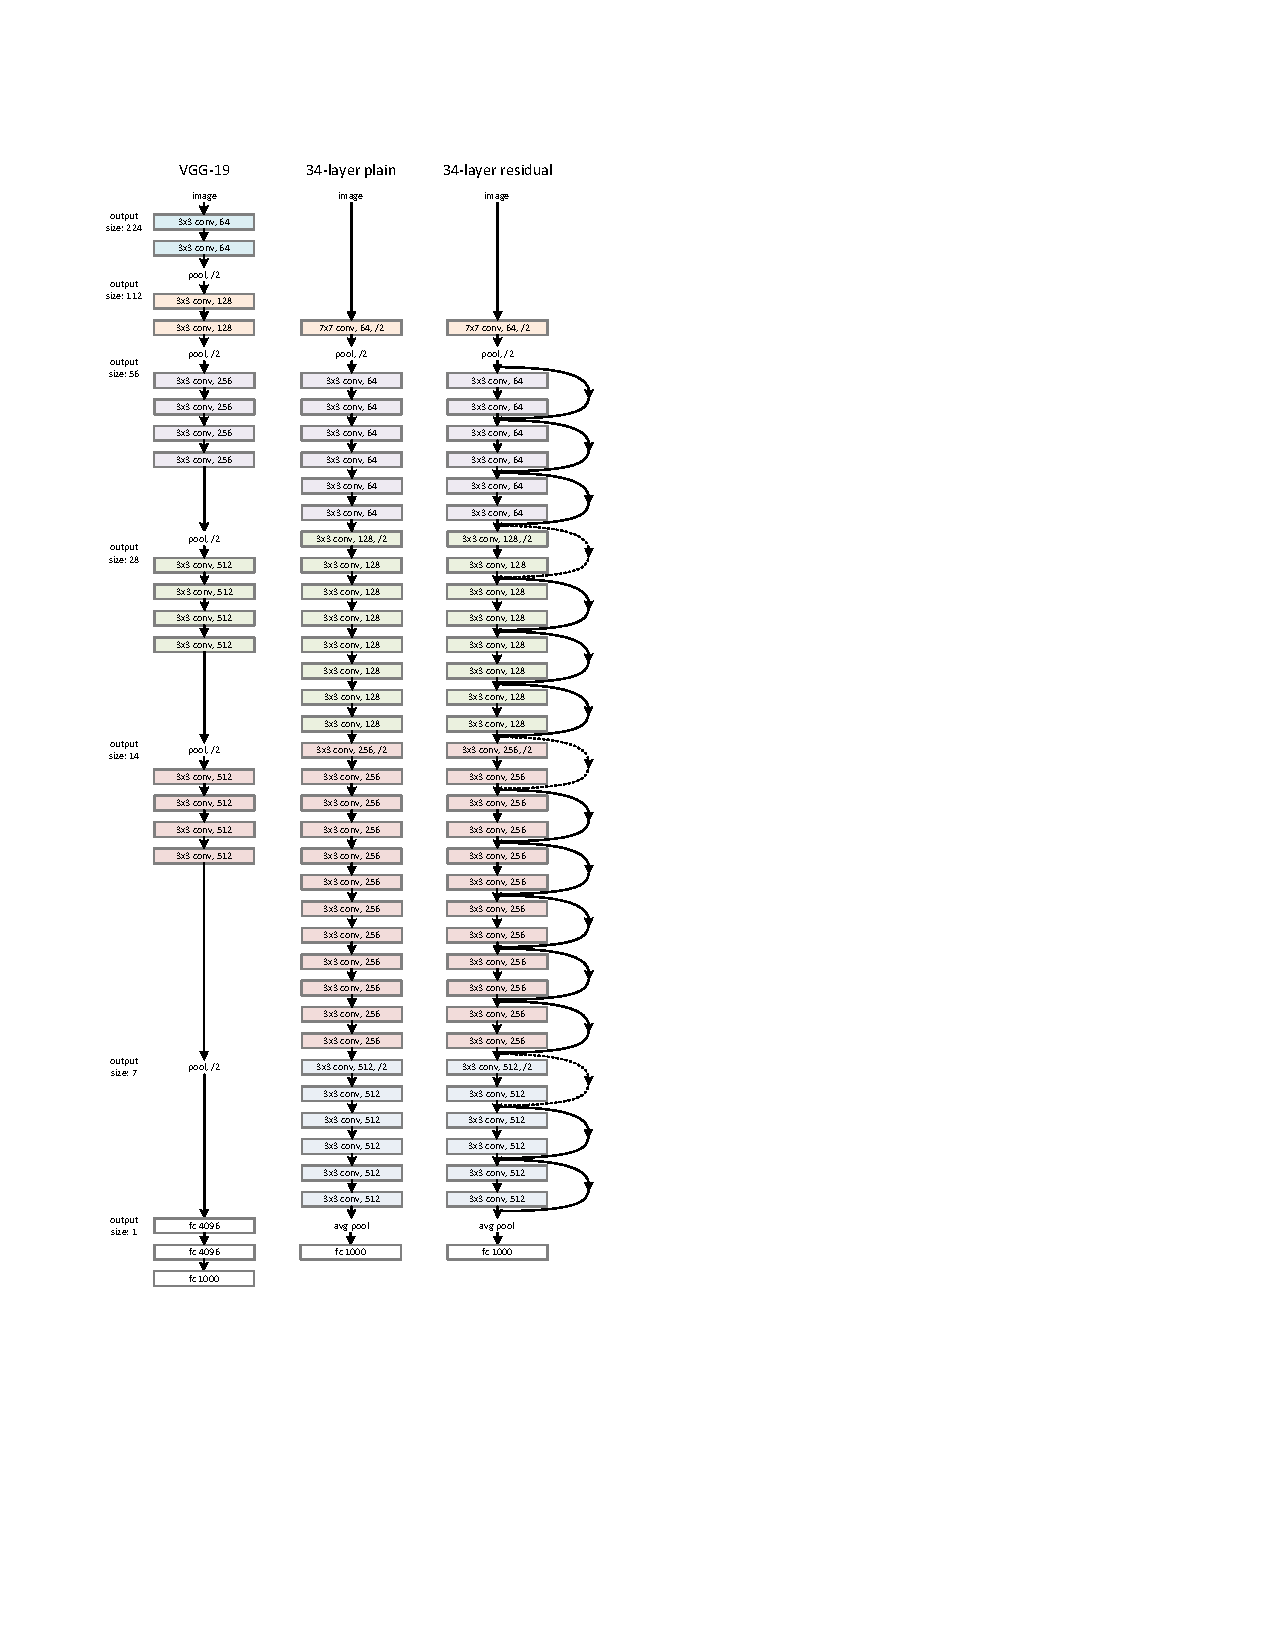
\includegraphics[width=\textwidth]{resnet}
        \end{column}
    \end{columns}
\end{frame}

\begin{frame}
    \frametitle{Supervised learning}
    Machine learning problems/algorithms categorized as \alert{supervised} vs.\ \alert{unsupervised}

    \begin{block}{Supervised learning}
        \begin{itemize}
            \item Data represented as $\{(\x_i, \y_i)\}_{i=1}^n$, with $\x_i$ an input and $\y_i$ an output
            \item Given $\x$, predict $\y$
        \end{itemize}
    \end{block}
    \pause

    Supervised learning further split into: \\[1ex]
    \begin{columns}[t]
        \begin{column}{0.47\textwidth}
            \alert{Regression}: $\y$ continuous, e.g.
            \begin{itemize}
                \item $\x =$ (age, sex, race, weight, height, LDL, HDL, zip code, etc.), $y =$ life expectancy
                \item $\x =$ (stock price history, market conditions, interest rates, etc.), $y =$ tomorrow's stock price
            \end{itemize}
        \end{column}
        \pause
        \begin{column}{0.45\textwidth}
            \alert{Classification}: $\y$ discrete, e.g.
            \begin{itemize}
                \item $\x =$ lots of pixels, $\y =$ image label (cat, dog, etc.)
            \end{itemize}
        \end{column}
    \end{columns}
\end{frame}

\begin{frame}
    \frametitle{More supervised learning examples}

    Regression
    \begin{itemize}
        \item Text-to-speech: $\x =$ words, $\y =$ speech audio
        \item Denoising: $\x = \text{data} + \text{noise}$, $\y = \text{data}$
        \item Anomaly detection: $\x =$ (time, location, amount, type) of credit card purchase, $y = \Prob(\text{fraud})$
        \item Prognosis: $\x =$ conditions of existing medical condition, $y =$ expected remaining life
    \end{itemize}
    \pause

    Classification
    \begin{itemize}
        \item Speech-to-text: $\x =$ audio speech sample, $\y =$ words spoken
        \item Spell check: $\x =$ misspelled word, $\y =$ intended word
        \item Machine translation: $\x =$ a sentence in English, $\y =$ the sentence in French
        \item Recommender problem: $\x =$ list of movies you like/dislike, $y =$ whether you like \emph{Interstellar}
        \item Diagnosis: $\x =$ your complete medical record, $\y =$ what medical condition(s) you have
    \end{itemize}
\end{frame}

\begin{frame}
    \frametitle{Converting classification to regression: one-hot}

    Classification problems almost always converted to regression via easy trick

    \begin{block}{One-hot encoding}
        For labels $1, \dots, n$, represent each label as the unit vector $\e_i$, $i = 1, \dots, n$ \\[1ex]
    \end{block}
    \pause

    One-hot vectors loosely interpreted as
    \begin{equation*}
        \begin{bmatrix}
            \Prob(\text{label} = 1) & \cdots & \Prob(\text{label} = n)
        \end{bmatrix}
    \end{equation*}

    E.g. image classification: \\[0.5ex]

    \centering
    \begin{tabular}{c|cc}
        label & index & one-hot vector \\
        \hline
        bird & 1 & $\begin{bmatrix} 1 & 0 & 0 & 0 & \cdots & 0 \end{bmatrix}$ \\
        cat & 2 & $\begin{bmatrix} 0 & 1 & 0 & 0 & \cdots & 0 \end{bmatrix}$ \\
        dog & 3 & $\begin{bmatrix} 0 & 0 & 1 & 0 & \cdots & 0 \end{bmatrix}$ \\
    \end{tabular}
\end{frame}

\begin{frame}
    \frametitle{Converting classification to regression: softmax}
    One-hot works for labeling data.
    What about model outputs?

    \begin{block}{Softmax activation}
        Converts arbitrary real vector (called \textcolor{blue}{logits}) to \textcolor{Green4}{vector of probabilities that sums to 1}
        \vspace{-1pt}
        \begin{align*}
            \softmax &: \textcolor{blue}{\Reals^n} \to
            \textcolor{Green4}{(0, 1)^n \text{ with } L^1 \text{ norm} = 1} \\
            &\hspace{1.25ex} \textcolor{blue}{%
                \left(\begin{bmatrix} y_1 & \cdots & y_n \end{bmatrix}\right)%
            } \mapsto
            \textcolor{Green4}{%
                \frac{1}{\sum_{i=1}^n e^{y_i}}
                \begin{bmatrix}
                    e^{y_1} & \cdots & e^{y_n}
                \end{bmatrix}%
            }
        \end{align*}
        \vspace{-10pt}
    \end{block}
    \pause

    Like one-hot, output loosely interpreted as
    \begin{equation*}
        \textcolor{Green4}{%
            \begin{bmatrix}
                \Prob(\text{label} = 1) & \cdots & \Prob(\text{label} = n)
            \end{bmatrix}
        }
    \end{equation*}
    (Real statisticians object to calling these \emph{probabilities}; we'll be flexible)

    \begin{itemize}
        \item E.g.: model outputs \textcolor{blue}{%
            logits
            $\y = \begin{bmatrix} -3.33 & 9.62 & 9.18 & \cdots \end{bmatrix}$
        }
        \item \textcolor{Green4}{%
            $\softmax(\y) = \begin{bmatrix} 1.40 \cdot 10^{-6} & 0.593 & 0.381 & \cdots \end{bmatrix}$
        }
        \item Model is 59.3\% confident in ``cat,'' 38.1\% confident in ``dog''
    \end{itemize}
\end{frame}

\begin{frame}
    \frametitle{Converting classification to regression: sigmoid}
    If $\exists$ only two classes (e.g., yes/no), second probability is redundant.
    Alternative:

    \begin{columns}
        \begin{column}{2.3in}
            \begin{block}{Standard logistic activation}
                Converts arbitrary real scalar (called \textcolor{blue}{logit}) to single probability
                \begin{align*}
                    \sigma &: \textcolor{blue}{\Reals} \to \textcolor{Green4}{(0, 1)} \\
                    &\hspace{1.25ex} \textcolor{blue}{y} \mapsto
                    \textcolor{Green4}{\frac{1}{1 + e^{-y}}}
                \end{align*}
            \end{block}
        \end{column}
        \begin{column}{1.8in}
            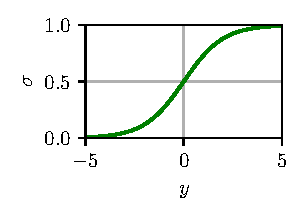
\includegraphics{sigmoid}
        \end{column}
    \end{columns}
    \vspace{1em}
    \pause

    Loose interpretation: $\Prob(\text{yes}) = \sigma(y)$, $\Prob(\text{no}) = 1 - \sigma(y)$

    \begin{itemize}
        \item Technically, any function of this shape is called ``sigmoid''
        \item Many people use ``sigmoid'' to refer specifically to the standard logistic
    \end{itemize}
\end{frame}

\begin{frame}[t]
    \frametitle{Unsupervised learning}
    \begin{block}{Unsupervised learning}
        \begin{itemize}
            \item Data represented as $\{x_i\}_{i=1}^n$ only: no outputs
            \item \alert{Density estimation}: learn the data's probability distribution
        \end{itemize}
    \end{block}

    \uncover<2->{Related problem: \alert{clustering}---find which clusters data belong to} \\[1ex]

    \uncover<4->{Examples:}
    \begin{itemize}
        \item<4-> Generative modeling: given \textcolor<5->{blue}{pictures of volcanoes}, generate \textcolor<5->{Green4}{new ones that look realistic}
        \item<6-> Determine if loan/insurance applicant is low/medium/high-risk
    \end{itemize}

    \temporal<2>{%
    }{%
        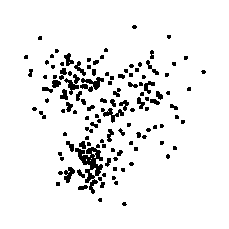
\includegraphics{cluster}%
    }{%
        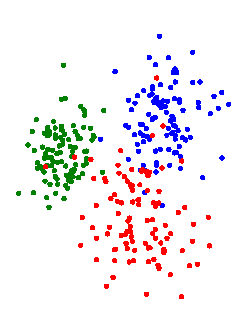
\includegraphics{clusters}%
    }
    \hfill
    \begin{tikzpicture}[
        node distance=5mm,
        frame/.style={draw, rectangle, ultra thick, inner sep=1pt}
    ]
        \visible<4->{
            \node (real) [frame, temporal=<5>{white}{blue}{blue}] {
                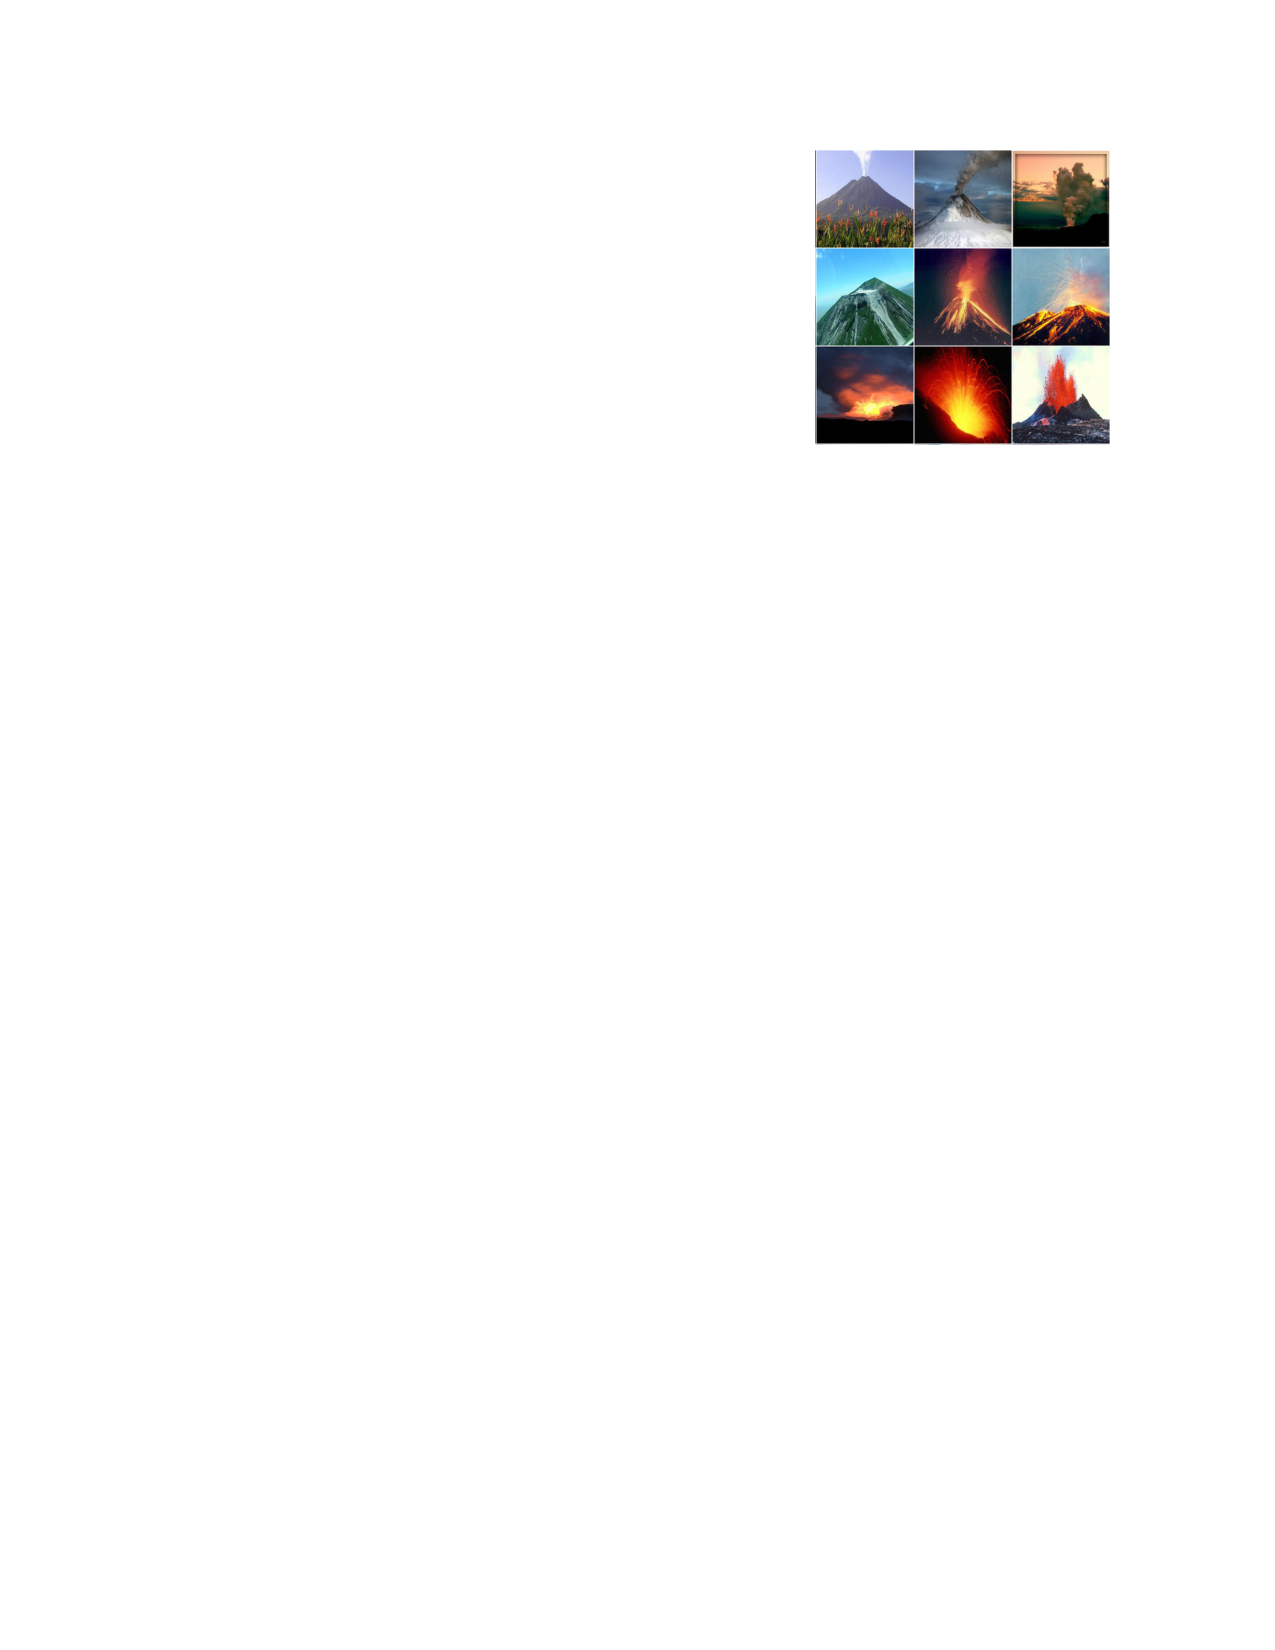
\includegraphics[width=3.2cm]{volcano_data}
            };
            \node (gen) [right=of real, frame, temporal=<5>{white}{Green4}{Green4}] {
                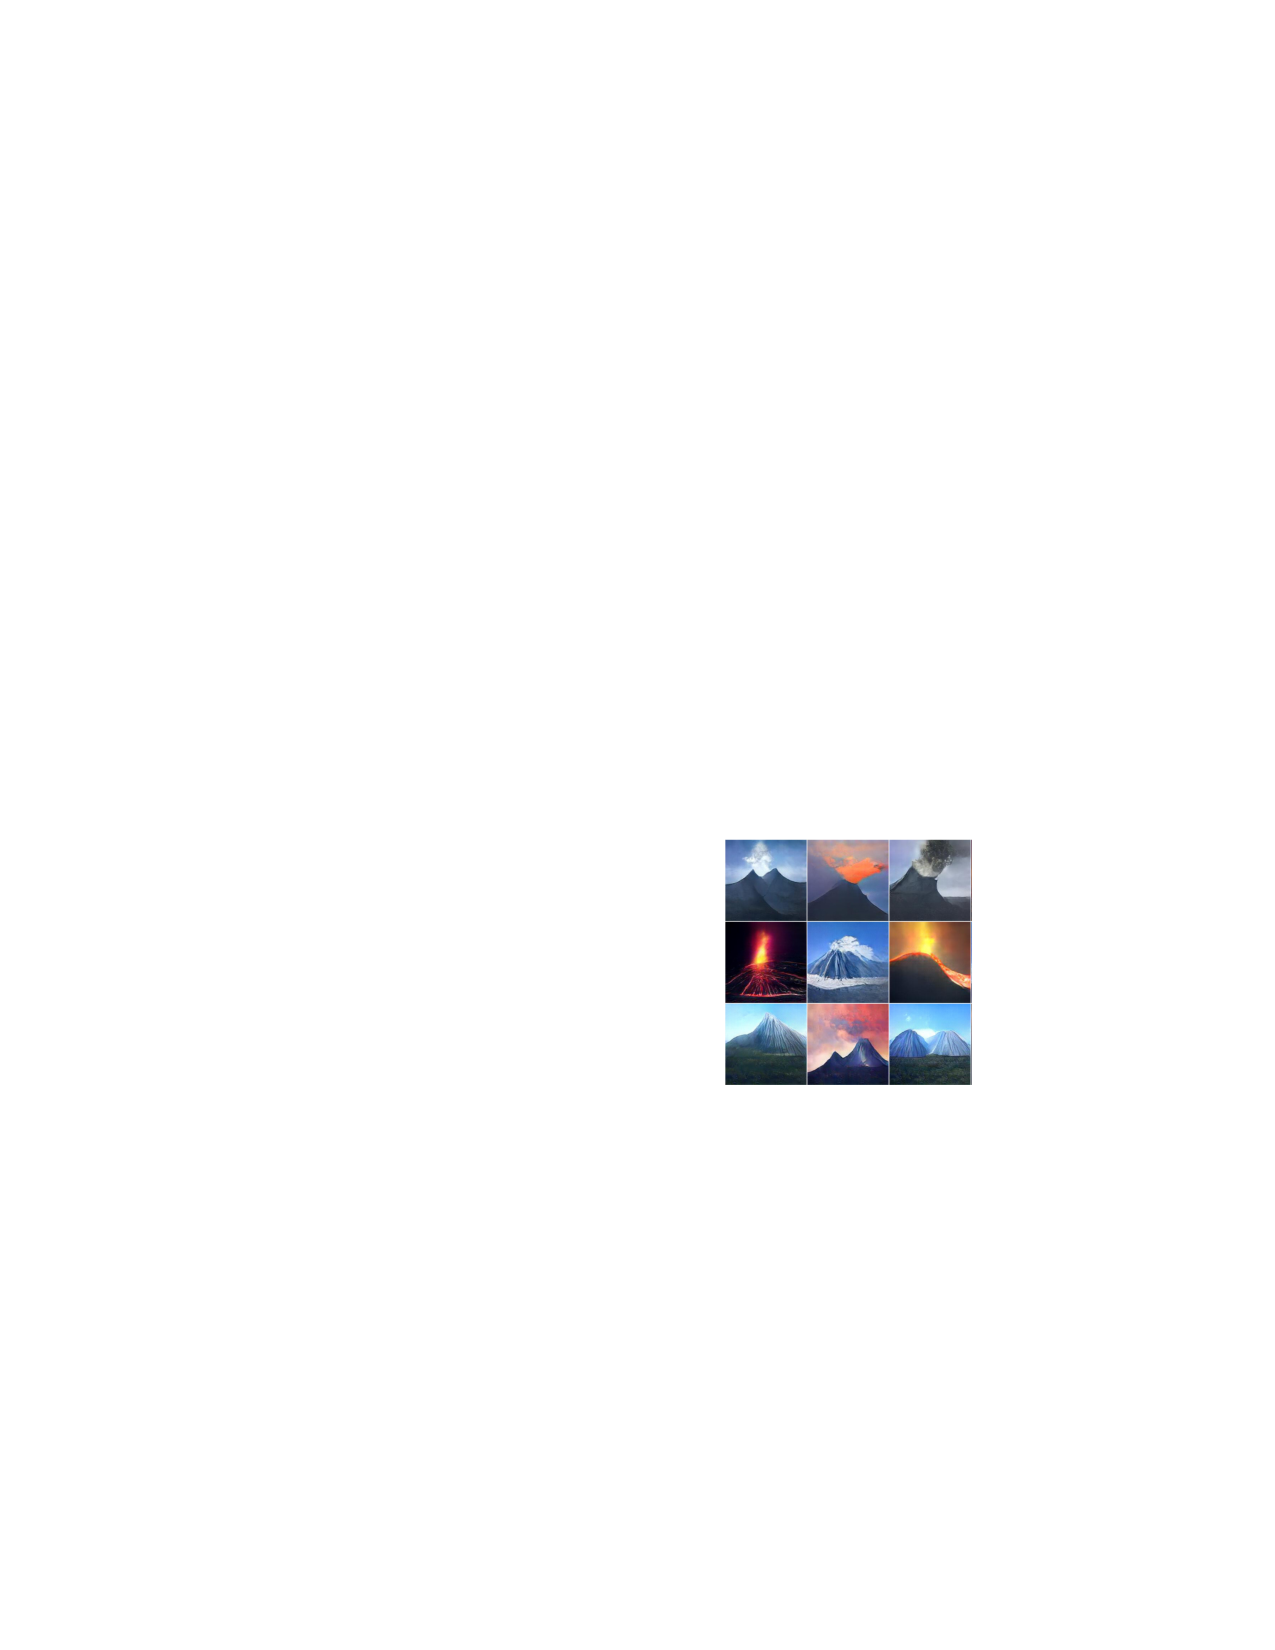
\includegraphics[width=3.2cm]{volcano_generated}
            };
        }
    \end{tikzpicture}
\end{frame}

\begin{frame}
    \frametitle{Notes on supervised vs.\ unsupervised learning}

    \begin{itemize}
        \item I will only focus on supervised learning today \& Thursday
        \begin{itemize}
            \item Theory more mature
            \item Techniques more powerful
        \end{itemize}
        \item Many experts believe a strong future in ML requires a shift toward unsupervised learning
        \begin{itemize}
            \item $\exists$ tons of data in the world, but often unlabeled
        \end{itemize}
        \item Semi-supervised learning: usually, small amount of labeled data + lots of unlabeled data
    \end{itemize}
\end{frame}

\begin{frame}
    \frametitle{Machine learning algorithms}

    \begin{columns}
        \begin{column}{0.44\textwidth}
            The list is long:
            \begin{itemize}[<.->]
                \item Logistic regression
                \item Gaussian mixture models
                \item Kernel methods
                \item Naive Bayes classifier
                \item $k$-nearest neighbors, $k$-means, $k$-medians
                \item Decision trees
                \item Random forests
                \item Support vector machines
                \item \alert<2->{(Artificial) neural networks}
                \item Etc.
            \end{itemize}
        \end{column}

        \begin{column}{0.56\textwidth}
            \uncover<2->{%
                I will only focus on neural networks.
                Even then, variations are plentiful:
            }
            \begin{itemize}[<2->]
                \item \alert<3->{Dense (fully-connected) NN: generic}
                \item Convolutional NN: for spatial data
                \item \alert<3->{Recurrent NN: for temporal data (Thursday's topic)}
                \item Autoencoders: for data representations
                \item Reinforcement learning: for AI/games
                \item Generative models: for making new data
                \item Recommender systems
                \item Etc.
            \end{itemize}
            \uncover<2->{These can generally be combined freely}
        \end{column}
    \end{columns}
\end{frame}

%%% Local Variables:
%%% mode: latex
%%% TeX-master: "../nn"
%%% End:
